\chapter{Бойна система}

\section{Детайлност}
В зависимост от сюжетните нужди, една схватка може да бъде описана в еднинствено изречение или на десетки страници.
За това настоящата глава е организирана както следва.
Дефинирани са голям брой правила, всяко с уникално име.
Следващите таблици описват кои правила се препоръчва да бъдат ползвани кога.
\\
% Represent each abstraction as a separate table.
\newenvironment{abstractiontable}[1]
{
  \rowcolors{1}{white}{lightgray}
  \noindent
  \textbf{#1}
  \\
  \begin{tabular}{ p{3cm} | p{3cm} | p{3cm} | p{3cm} | p{3cm} }
}
{ \end{tabular} }

\begin{abstractiontable}{Петте нива на абстркция}
Детайлно                  & Индивидуално & Строево        & Стратегическо                                   & Опростено  \\
максимална реалистичност  & a la DnD     & a la Total War & решава съдбата на армии с едно хвърляне на зар  & изчислително леко и универсално  \\
2-6 участници в схватката & 2-20         & 20-10000       & 20-много                                        & 2-20  \\
\end{abstractiontable}

\begin{abstractiontable}{Ръкопашен сблъсък}
байнд                    &                    &                &                                                &        \\
боравене                 & боравене           &                &                                                &        \\
две оръжия               &                    &                &                                                &        \\
дистанция                &                    &                &                                                &        \\
джаб                     &                    &                &                                                &        \\
удар по крайник          &                    &                &                                                &        \\
финт                     &                    &                &                                                &        \\
изисквана сила           & изисквана сила     &                &                                                &        \\
свойства на оръжие       & свойства на оръжие &                &                                                &        \\
типове щети              &                    &                &                                                &        \\
щети                     & щети               &                &                                                &        \\
                         &                    & нападение      & ???                                            & бонус  \\
\end{abstractiontable}

\begin{abstractiontable}{Стрелба}
автоматична стрелба      & автоматична стрелба &                    &                                                &        \\
изстрел                  & изстрел             &                    &                                                &        \\
лесни оръжия             & лесни оръжия        &                    &                                                &        \\
обсег                    & обсег               & обсег              &                                                &        \\
прицелване               &                     &                    &                                                &        \\
стрелба по крайник       &                     &                    &                                                &        \\
                         &                     & обстрел            & ???                                            &        \\
\end{abstractiontable}

\begin{abstractiontable}{Отбрана}
покритие като лук        & покритие - число &                &                                                &  \\
пазене                   & пазене           &                &                                                &  \\
                         &                  & отбрана        &                                                &  \\
\end{abstractiontable}

\begin{abstractiontable}{Ресурси}
ранa                     & ЖТ       & здрави/ранени  & хора                                           &  \\
\end{abstractiontable}

\begin{abstractiontable}{Придвижване}
                         &          &                & придвижвне на армия                            &  \\
езда, шофиране           &          &                & придвижвне на армия                            &  \\
\end{abstractiontable}

\begin{abstractiontable}{Морал}
                         &          & морал          &                                                &  \\
\end{abstractiontable}


\section{Списък с правила}
\subsection{Автоматична стрелба}
Автоматичните оръжия са способни да произведат повече от един изстрел за ход.
Хвърлянето за атака е едно и броят изстрели се заявява предварително.
Всеки изстрел след първия има <откат> точки по-малко атака, натрупвайки се.


\subsection{Байнд}
Наместо атакуване с ръкопашно оръжие, войн може да опита да постигне доминантна позиция в байнд.
Това изисква двамата войни да са на дистанция, в която поне единият може да удари другия.
Следващия ход нападателят има +5 на боравене.


\begin{multicols}{2}
\subsection{Боравене}
Число, описващо колко вероятно е ръкопашна или далечна атака да достигне целта си.
Равно е на умението с използвното оръжие.
\\
\\
Ръкопашна атака може да бъде парирана от врага с число, равно на тяхното боравене.
Алтернативно, атаката може да бъде отбегната акробатично, с число (Ловкост-5), но ако следващия ход бъде извършена контраатака, тя има бонус +5(нaпадателят се е открил).
\\
\\
Ако нападението е поне равно на отбраната, удар е пласиран, но може да бъде спрян от броня.


\subsection{Две оръжия}
Едното оръжие се ползва за да нанесат щети на врага, нека наречем него първо.
Второто оръжие може да се ползва за създаване на откриване (което добавя половината боравене в това оръжие към боравенето с основното оръжие) или пък независимо, за пласиране на стопиращи удари (в който случай се ползва независимо, но с наказание -5 на атака).
Ако се атакува само с едното оръжие няма наказания, разбира се.
Щитовете не търпят -5 при пазене.
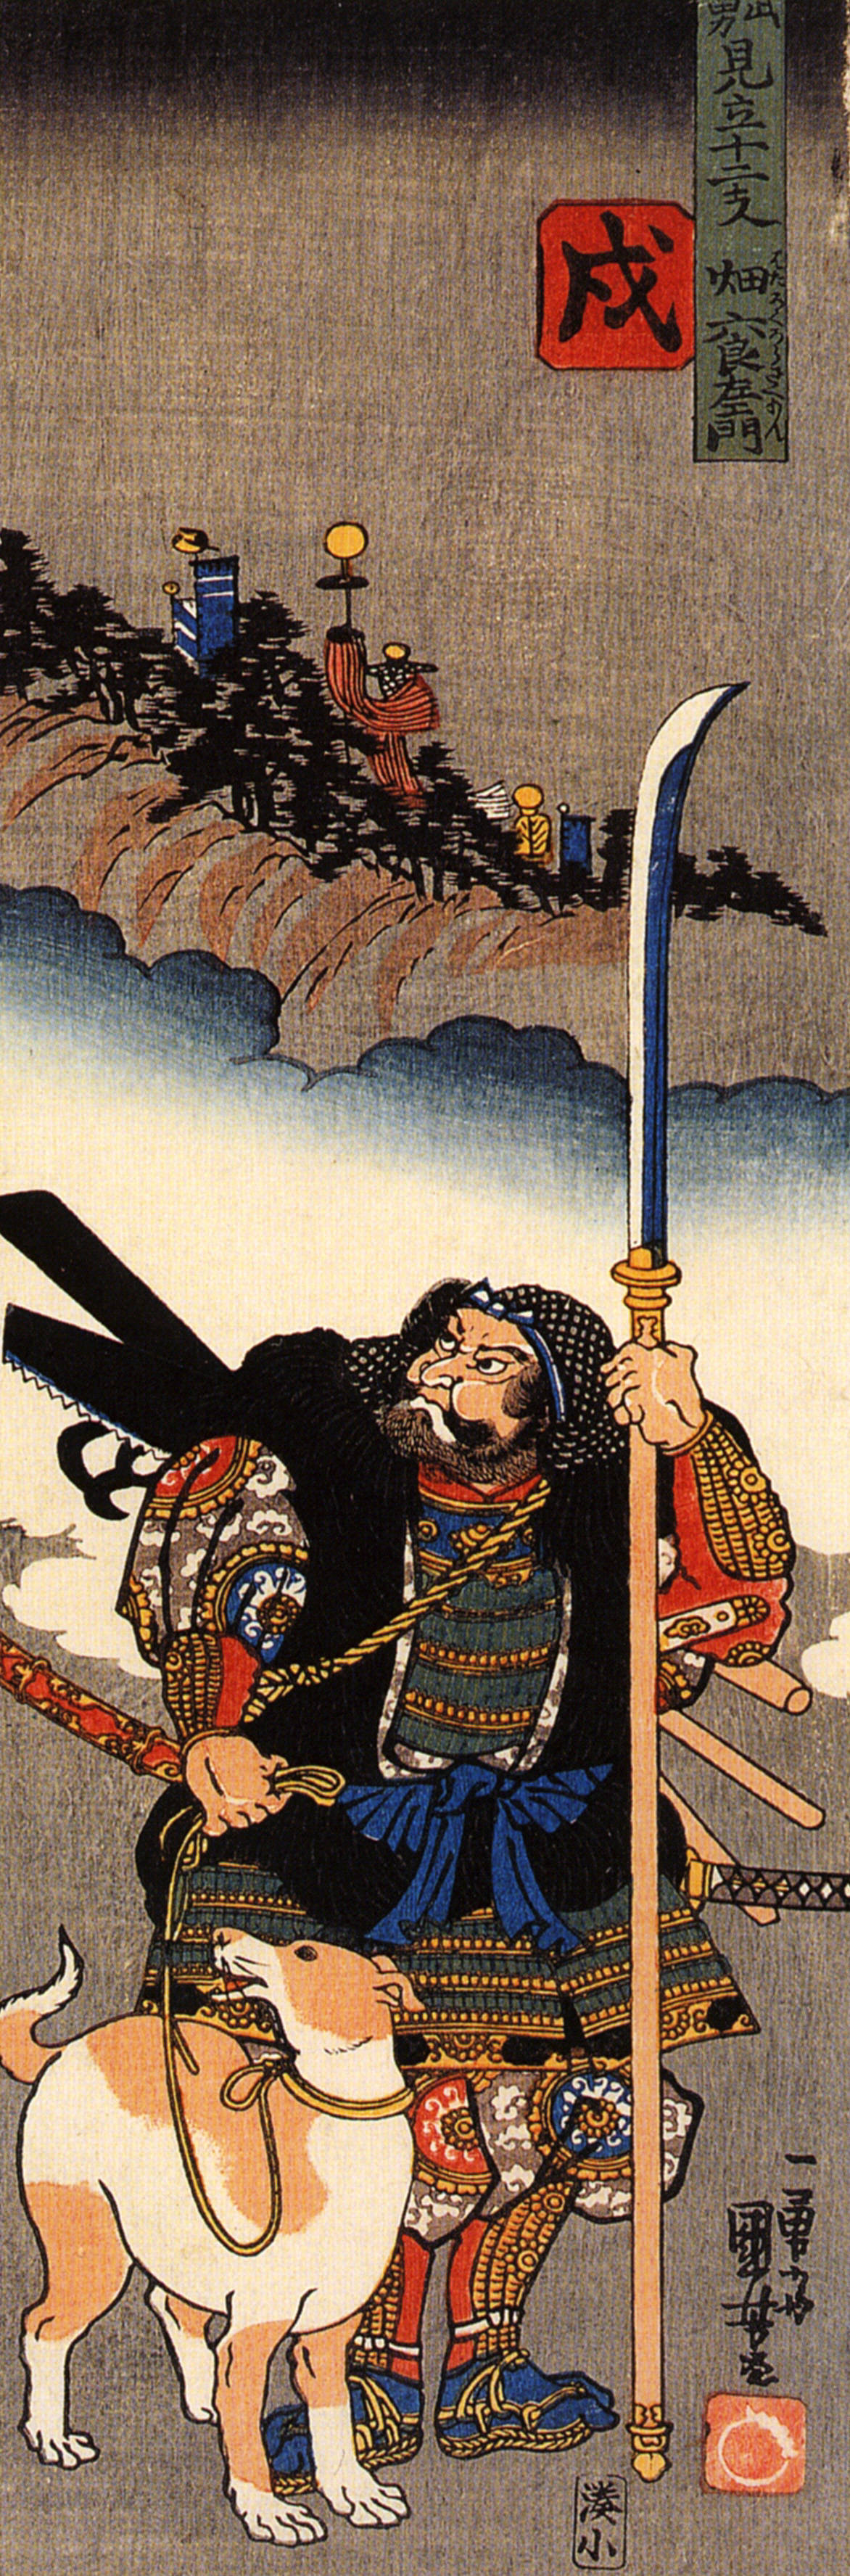
\includegraphics[height=0.8\textheight]{../images/naginata}~


\subsection{Дистанция}
\begin{enumerate}
\item{директна (борба)}
\item{близка (нож, невъоръжен, къс меч)}
\item{средна (меч 80см, повечето оръжия за една ръка)}
\item{дълга (дълъг меч, копие, двуръчен меч)}
\item{отдалечена (пика)}
\item{извън ръкопашен обхват (стрелящи неща)}
\end{enumerate}
Инициатива за първия удар има този с по-дълго оръжие (очевидно).
Извън оптималната си дистанция, оръжията са на -5 атака и половин щети.
Придвижване между дистанции се извършва след успешно хвърляне (независимо нападение или защита).
Придвижването е или една категория в произволна посока или произволен брой категории, без да се преминава през заплашвани от някой враг дистанции.
\\
\anexample{Пешо, с копие и нож, напада Жоро, с меч.
Пешо връхлита и напада с копието.
Хвърля боравене + d6* < боравене на Жоро.
Жоро е отбягнал атаката и може да промени дистанцията.
Пешо заплашва дълга (копие една ръка) и близка(нож)
Жоро може да избере близка, средна, дълга, отдалечена или да побегне.}


\subsection{Джаб}
Това е бърза ръкопашна атака, която избягва откриване или дисбалансиране на себе си.
Ползва (боравене+5), но причинява (Щ/2).
\end{multicols}


\subsection{Езда, Шофиране}
Ползване на умения от гърба на кон е ограничено до нивото на езда.
Например при боравене с копие 6 и езда 4, нападението е 4 + *d.
\\
\\
Ръкопашни атаки от и по галопиращ конник са с двойни щети.
Цялото тяло на конник, изключае краката и коня, са на 1 категория дистанция по-далеч от пешаци.
Съответно краката на пешаци са на една категория по-далеч от конник.
\\
\\
Стрелба от галопиращ кон, освен горното ограничение, търпи (модификация-10+езда), която модификация не може да е положителна.
\\
\\
Друго приложение на умела езда е бързо придвижване през труден терен или по улици със завои.


\subsection{ЖТ}
Жизнените точки са равни на Сила.
Ако бъдат бъдат редуцирани до или под 0, съществува опасност от безсъзнание или смърт.
При всяка рана, която резултира в ЖТ <=0, се хвърля зар.
5 -> смърт, 3 -> безсъзнание и смъртоносна рана, 1 -> безсъзнание


\subsection{Необходима сила}
Това е обсегът на Сила на героят, в който оръжието е ефективно.
Ако персонажът има по-малко от минималната сила, разликата става наказание върху боравенето с това оръжие.
От друга страна, Сила, по-висока от максималната, не допринася за по-високи щети.


\subsection{Изстрел}
Тук спадат всички далечни оръжия без автоматичен режим на стрелба като лък, арбалет, пистолет и дори франциска или просто камък.
\\
\\
\rowcolors{1}{white}{lightgray}
\begin{tabular}{l | l | l | l }
Ситуация         & Трудност & Модификация & Бележки                                                    \\
неподвижен човек & 0        & -           &                                                            \\
следящ оръжието  & Ловкост  & -           & струва цял ход                                             \\
тичане           & -        & +5          &                                                            \\
в ръкопашен бой  & -        & +5          & при пропуск се хвърля срещу останалите учасници в клането  \\
\end{tabular}


\subsection{Лесни оръжия}
Някои оръжия, като арбалетът или повечето огнестрелни оръжия, могат да бъдат ползвани след само ден тренировки.
С тях може да бъде нападано ползвайки Ловкост, наместо боравене.
Твоа важи само за нападение - боравене е нужно за Прицелена стрелба, ремонтиране, ползване ранен и така нататък други действия.


\subsection{Многобой}
Това е ситуация, в която един войн е в ръкопашен бой с няколко врага.
Тогава той има право само на една отбрана на ход като париране или отбягване, и има трудност да бъде уцелен 0 срещу всички останали нападение.
Алтернативно, той може да отдели някои точки от основната си отбрана за последващи такива.
Примерно мечоносец с боравене 8 може да реши да се предпази от двамата си опоненти с (4 + d*), наместо от първия с (8 + d*) и от втория с (d*).


\subsection{Нападение на строй}
нападение = (боравене + средни Щ (+ 5 за конник)) / 2


\subsection{Обсег}
За стрелящи оръжия.
Най-голямото разстояние, на което стрелецът може да се прицели с лекота.
През всеки инкремент метра, атаките търпят по -5 наказание.


\subsection{Обстрел на строй}
обстрел = (боравене + средни Щ (+5 за автоматични оръжия)) / 2


%\subsection{Обща абсорбация}
%общо покритие = (покритие глава + покритие торс + покритие ръце + покритие крака) / 4
%\\
%обща абсорбация = (аб + общо покритие) / 2


%\subsection{Отбрана на строй}
%отбрана = (боравене + обща абсорбация)


\subsection{Пазене}
Свойството на броня да абсорбира част от сериозността на удар.


\subsection{Покритие(на броня)}
Всяко парче броня има асоцирано число 'покритие', описващо колко пълно покрива тялото.
Най общо, хвърлянето за боравене на нападател трябва да надвие боравене + прикритие за да заобиколи бронята. 
юю
Парчета броня могат да бъдат носени заедно или едно под друго.
\begin{itemize}
\item{на главата може да бъде носен шлем върху бронирана качулка}
\item{на торса може да бъде носен нагръдник върху ризница и гамбезон; или плочи върху бронежилетка}
\item{на ръцете могат да бъдат носени нараменници, налакътници и ръкавици върху бронирани ръкави}
\item{на краката могат да бъдат носени бронирана пола, набедреници, наколенки, грейвси върху бронирани крачоли}
\end{itemize}

Колкото по-голяма е разликата при хвърлянето за уцелване, толкова по-вероятно е да е уцелено слабо място в бронята, заобикаляйки я частично или напълно.
Брони една върху друга действат независимо една от друга.
\\
\anexample{
Нагръдник с покритие 5 върху ризница с покртитие 10.
\\
\rowcolors{1}{white}{lightgray}
\begin{tabular}{ p{8cm} | p{8cm} }
боравене на нападателя + d* >= боравене на отбраняващият се + 10 & всичката броня е заобиколена  \\
боравене на нападателя + d* >= боравене на отбраняващият се + 5  & нападението заобикаля нагръдника, но попада в ризницата  \\
боравене на нападателя + d* >= боравене на отбраняващият се      & нападението попада в нагръдника, и ако той не го спре- в ризницата  \\
\end{tabular}
}
\\
От друга страна, някои парчета боня се носят заедно.
\\
\anexample{Ръкавици с покритие 4 и налакътници с покритие 3 представляват една броня за ръцете с покритие 7 и пазене средно аритметично от двете.}


\begin{multicols}{2}
\subsection{Прицелване}
Това действие е възможно, когато се ползва изцяло стрелящо оръжие като арбалет или пушка, но не и лък или ръчна граната.
То може да бъде извъшено толкова пъти, колкото е (боравене) със съответното оръжие.
Всеки ход, прекаран в прицелване, добавя +1 модификация.
След това целта може да бъде следена, запазвайки модификацията, докато нещо съществено се промени: влезе в автомобил, легне, затича се.


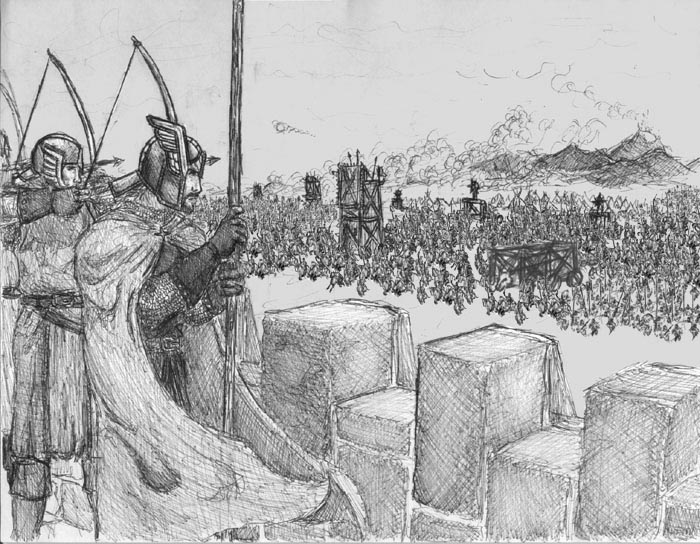
\includegraphics[width=0.6\textwidth]{../images/siege}~


\subsection{Прикриване}
Прикритие от ръкопашни атаки, като зад тезгях или зад ъгъла, дава (боравене+5) за целите на отбрана и на двамата опоненти.
\\
\\
Когато става дума за стрелба, концепцията е далеч по-важна и ефективна.
Следната модификация се вади от боравенето на враг, стрелящ по прикрития персонаж.
\\
\rowcolors{1}{white}{lightgray}
\begin{tabular}{p{2cm} | p{1cm} | p{5cm}}
Ситуация        & Модификация & Бележки \\
полу-прикритие  & -5          & поне половината тяло е скрито, примерно зад крепостна стена или заложник \\
пълно прикритие & -10         & примерно зад ъгъла; атаки търпят -5 наказание                            \\
\end{tabular}
\end{multicols}

 
\subsection{Ранa}
След като нападение премине през бронята, делим оставащите точки щети на Сила на ранения:
\\
\\
\rowcolors{1}{white}{lightgray}
\begin{tabular}{ p{3cm} | p{3cm} | p{3cm} | p{3cm} | p{3cm} }
Сериозност & ръка                                                                             & крак                                                                            & торс                                     & глава                                                   \\
>=0        & -                                                                                & -                                                                               & -                                        & o: -5 заради кръв в очите т: следващият ход се пропуска \\
>=0.5      & о: кървене т: неизползваема 10 мин                                               & о: кървене т: поваляне                                                          & о: кървене т: следващият ход се пропуска & -5 и слдващият ход се пропуска     \\
>=1        & о: кървене, срязани сухожилия, мускули и/или нерви т: кървене, открита фрактура  & о: кървене, срязани сухожилия, мускули и/или нерви т: кървене, открита фрактура & о: обилно кървене(перфориран бял дроб или изсипан корем) т: натрошени ребра(каквото и да е движение води до перфориран бял дроб)                 & шок, обилно кървене(черепът е пробит) \\
>=2        & о: отрязана т: откъсната                                                         & о: отрязан т: откъснат                                                          & унищожено сърце и/или врат                                                       & о: отсечена т: унищожена \\
\end{tabular}

\noindent
Кървене: натрупваща се модификация -1/ход.
Дишането е проверка за сила с трудност -20.
\\
\\
Обилно кървене: -5/ход.
\\
\\
Остри щети се случват когато мушкаща или сечаща атака изцяло заобиколи бронята.
\\
\\
Шок се причинява от прекомерна кръвозагуба или хидравличен шок.
Симптомите са незабавно безсъзнание докато причинителят не бъде отстранен.


\subsection{Стрелба по крайник}
\rowcolors{1}{white}{lightgray}
\begin{tabular}{l | l | l | l }
глава & модификация -5  \\
торс  & -  \\
ръка & модификация -5  \\
крак & модификация -5  \\
\end{tabular}


\subsection{Свойства на оръжие}
\begin{itemize}
\item{\textit{повратливост} - покрива всички по-близки дистанции от максимлната}
\item{\textit{бронебойност} - пренебрегва половината пазене на целта}
\item{\textit{трудно за вадене} - не може да се извади от пробита броня, щит или плът; при вадене лечитеслтво с/у щетите; ако не успее се  нанасят още толкова щети, колкото първоначално}
\item{\textit{поваляне} - наместо щети оръжието спъва и поваля опонента, дори конник; качествено бойно седло дава -5 на атака}
\item{\textit{обезоръжащи куки} - ако париране със съответния щит или оръжие надхвърли с 5 нападението, вражеското оръжие е хвърлено на земята}
\item{\textit{закачане на щит} - наместо щети, обръща вражеския щит така че да не пази; продължава до следващата атака на врага; не пречи на офанзивата със щит}
\end{itemize}


\subsection{Удар по крайник}
\rowcolors{1}{white}{lightgray}
\begin{tabular}{l | l | l | l }
глава & -  \\
торс  & -  \\
ръка  & може да бъде извършена на една дистанция по-далеч от нормално  \\
крак  & -  \\
\end{tabular}


\subsection{Типове щети}
Мушакщи атаки (Щм) са бързи, но оставят нападателя открит за контраатака(боравене-5 следващия ход).
Причиняват високa смъртност(Щ*2).
\\
\\
Сечащи атаки (Щс) постигат балнс между офанзива и отбрана, защото арката на удара действа като париране/щит.
\\
\\
Трошащи атаки (Щт) преминават през броня(аб/2).
Те обаче са бавни, съотeрно лесни за отбягване(боравене-5).
Заради инертността на оръжието, атаките са трудни за париране (боравене-5 за париране с остро оръжие).
Същото важи и в обратната ситуация(боравене-5 за париране на остро оръжие).


\subsection{Финт}
Финтът е хазарт.
Сравнява се (боравене с вражеското оръжие + d*) с/у (боравене на врага с нашето оръжие).
Ако е поне равно, се получава (боравене+5) до началото на следващия ход.
В настоящия ход може да се реализира и нормална атака.
Иначе се получава (боравене-5).


\subsection{Щети}
Щети от попадение с ръкопано оръжие зависят от Сила на ползвателя му според следната таблица.
Конктетното оръжие може да има модификации върху тази стойност.
\\
Стрелящи оръжия нанасят щети спрямо някаква фиктивна "Сила" на оръжието.
\\
%\begin{wraptable}[24]{l}{5.5cm}
\rowcolors{1}{white}{lightgray}
\begin{tabular}{l | c | c | c}
     & ниски & средни & високи  \\
Сила & *1/2  & *2/3   & *1      \\
1  & d-3  & d-3  & d-2   \\
2  & d-3  & d-2  & d-1   \\
3  & d-2  & d-1  & d-1   \\
4  & d-2  & d-1  & d+1   \\
5  & d-1  & d    & d+2   \\
6  & d-1  & d    & d+3   \\
7  & d    & d+1  & 2d    \\
8  & d+1  & d+2  & 2d+1  \\
9  & d+1  & 2d-1 & 2d+2  \\
10 & d+2  & 2d   & 3d    \\
11 & d+2  & 2d   & 3d+1  \\
12 & 2d-1 & 2d+1 & 3d+2  \\
13 & 2d-1 & 2d+2 & 3d+3  \\
14 & 2d   & 3d-1 & 4d    \\
15 & 2d+1 & 3d   & 4d+1  \\
16 & 2d+1 & 3d+1 & 4d+2  \\
17 & 2d+2 & 3d+1 & 5d    \\
18 & 2d+2 & 3d+2 & 5d+1  \\
19 & 3d-1 & 4d-1 & 5d+2  \\
20 & 3d-1 & 4d   & 5d+3  \\
21 & 3d   & 4d   & 6d    \\
22 & 3d+1 & 4d+1 & 6d+1  \\
23 & 3d+1 & 4d+2 & 6d+2  \\
24 & 3d+2 & 5d-1 & 7d    \\
25 & 3d+2 & 6d   & 7d+1  \\
26 & 4d-1 & 5d   & 7d+2  \\
27 & 4d-1 & 5d+1 & 7d+3  \\
28 & 4d   & 5d+2 & 8d    \\
29 & 4d+1 & 6d-1 & 8d+1  \\
30 & 4d+1 & 6d   & 8d+2
\end{tabular}
%\end{wraptable}


%\subsection{Масови сражения}
%Групи от съюзници могат да бъдат събирани в "строй".
%Не е нужно групата да е хомогенна, но трябва да имат обща цел.

%\subsection{Характеристики на строй}
%\begin{itemize}
% Структурни
%\item{Лице - брой бойци с достъп до врага.}
%\item{Гъстота - от 1:1 (стена от щитове) до 1:5 (цвайхендери)}
%\item{Връхлитане - х1.5 за пешаци, х3 за конница}
%\item{Придвижване - равно на придвижването на най-бавният.}

% Състояние
%\item{Брой живи - бойци в добро здраве.}
%\item{Брой ранени - небоеспособни, в ръцете на лекарите след битка.}
%\item{Морал - равен на Дисциплина(У), спадне ли до 0, строят се превръща в "тълпа".}

% Компетентност и екипировка
%\item{Ръкопашен бой - Сила + най-високото боравене с налично ръкопашно оръжие.}
%\item{Стрелба - Сила + най-високото боравене с налично далечно оръжие}
%\item{Броня - Сила + (1/10)сума(пазене * здравина), без щитове}
%\end{itemize}
%\subsection{Правила}
%Ръкопашен бой + д6* с/у броня. Ако нападащият строй спечели, лицето на строят му се нанася 1/2 като убити и 1/2 като ранени върху противника. Разликата в хвърлянето се нанася върху моралът на противника / противника губи 1 точка морал (\textit{кое е по-добро?}).

%Директна стрелба (под 1 инкремент на оръжието) следва правилата за ръкопашен бой. Стрелба до максималното разстояние на хвърляне на оръжието е на половина щета.

%Лице и Дълбочина. Един строй може да бъде нападнат едновременно от най-много толкова строеве, сумата от чиито лица е колкото два пъти лицето на  нападнатите.

%Ако броят живи спадне под числото лице, строят се разпада (превръща се в тълпа).

%Ранените бойци са боеспособни, но намалят придвижването на стоя на половина. Лекуването им отнема половин месец.

%Морал. При виждане на разбиване на приятелски сторй, или ако бягащ разбит строй премине през позициите на друг строй, морал се намаля с 1.

%При морал 0, строят се разбива и се превръща в тълпа.

%Войници не в строй (а в тълпа) търпят наказание на всичко от -5.

%При виждане на поне двойно числено превъзхождащ противник, всеки строй губи 1 морал.

%При виждане на подготвящ се да връхлети двойно по-многоброен или много по-добре екипиран строй, строят губи 1 морал.

%Моралът се възстановява извън битка с 1 точка на минута.



%\subsection{здрави/ранени}
% Брой боеспособни войници с/у брой небоеспособни
% Ранените забавят армията, и някои от тях никога не се възстановяват


%\subsection{Придвижване на армия}
% фактори - статистики на хората, брой коне, размер на обоза



%\\
%\subsection{Напдение}
%TODO: reclim notes from Sofia.
%\\


% /subsubsection{Бонус}
% TODO: base upon notes from Sofia


%\subsection{Навесна стрелба}


